\section{Processamento de Imagens}


\subsection{Separação dos comprimidos}


A primeira etapa para extrair dados da imagem é isolar os comprimidos presentes. Para isso é preciso a conversão da imagem para escala de cinza, facilitando assim na utilização de operações de filtragem na imagem em etapas subsequentes. Para exemplificar a explicação daqui em diante utilizamos uma imagem do banco de dados, original na figura \ref{fig:proOrig}, e aplicando a conversão para escala de cinza temos o resultado na figura \ref{fig:proCinza}.

Em seguida, é necessário a detecção das bordas do comprimido. Como as imagens do banco de dados possuem um fundo padronizado o uso da técnica de limiar é possível. Um resultado possível pode ser observado na figura \ref{fig:proLim}. 

O próximo passo é eliminar resíduos da imagem deixando apenas o contorno do comprimido. Para isso são realizadas operações de abertura e fechamento utilizando elementos estruturantes circulares maiores que o resíduo e menores que o comprimido. Com isso obtemos uma máscara do exemplo utilizado, na figura \ref{fig:proMask}.

Por fim, uma técnica de detecção de objetos conectados é aplicada, a qual consegue separar objetos na imagem por meio de observação da vizinhança na imagem. Aplicando essa técnica nos exemplos temos o resultado nas figuras \ref{fig:proMask1} e \ref{fig:proMask2}.

Com a máscara segmentada é possível separar os comprimidos por meio de uma multiplicação com a imagem original, com isso obtemos as figuras \ref{fig:proPill1} e \ref{fig:proPill2}.

\begin{figure}[H]
        \centering
        \subfloat[][Original]{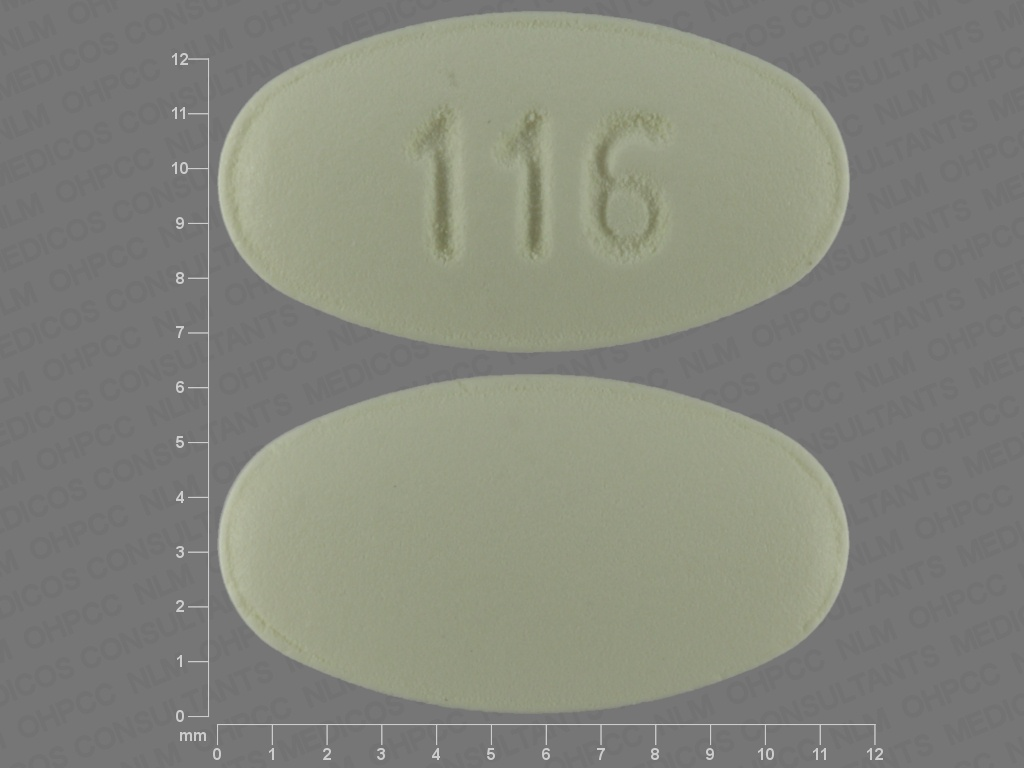
\includegraphics[width=0.3\textwidth]{figuras/processamento/original.jpg}\label{fig:proOrig}}
        %\hspace{0.1\textwidth}
        \subfloat[][Escala de cinza]{
        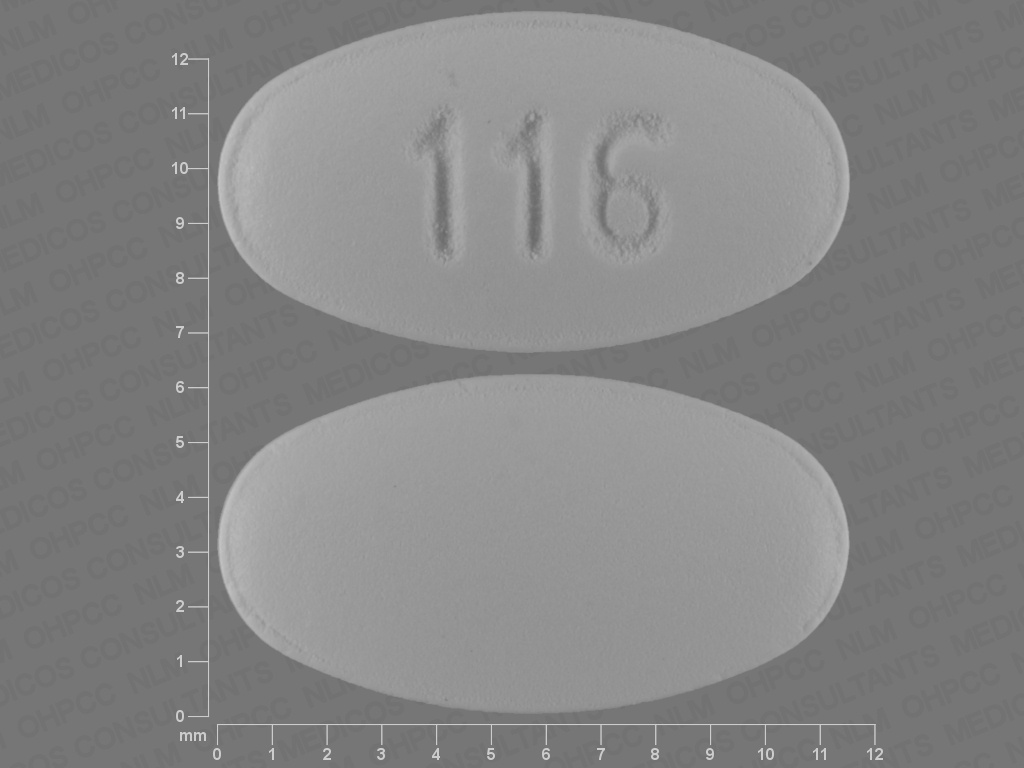
\includegraphics[width=0.3\textwidth]{figuras/processamento/cinza.jpg}\label{fig:proCinza}}
        \subfloat[][Limiar]{
        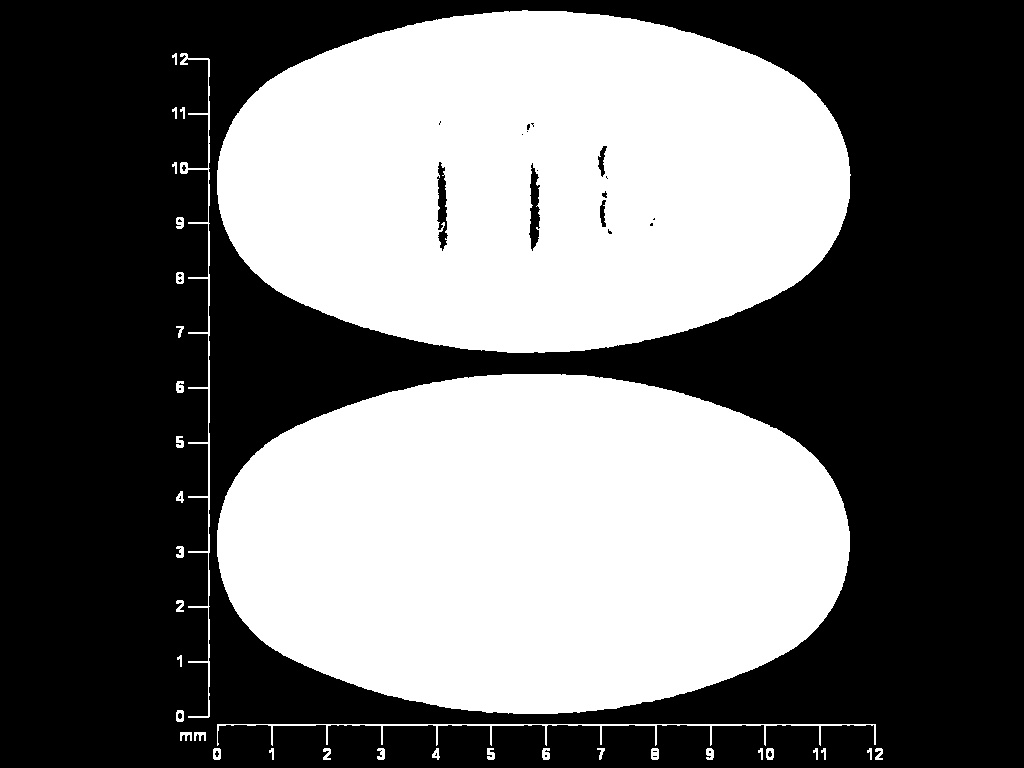
\includegraphics[width=0.3\textwidth]{figuras/processamento/limiar.jpg}\label{fig:proLim}}
        
        \subfloat[][Máscara]{
        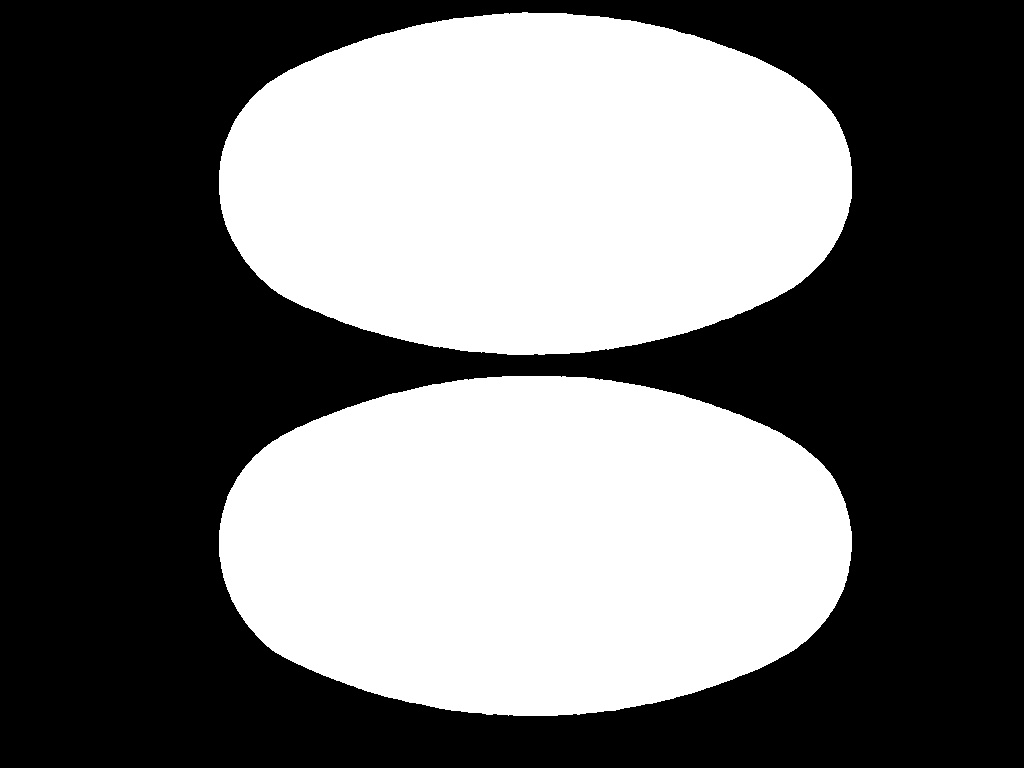
\includegraphics[width=0.3\textwidth]{figuras/processamento/mascara.jpg}\label{fig:proMask}}
        \subfloat[][Objeto 1]{
        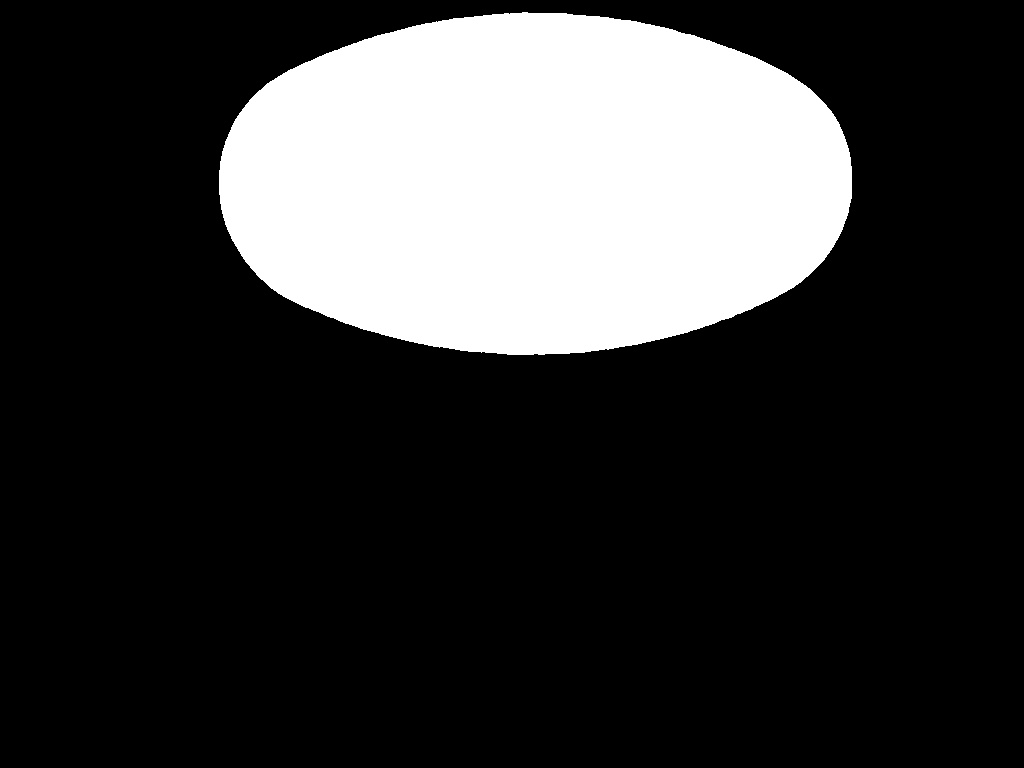
\includegraphics[width=0.3\textwidth]{figuras/processamento/mascara1.jpg}\label{fig:proMask1}}
        \subfloat[][Objeto 2]{
        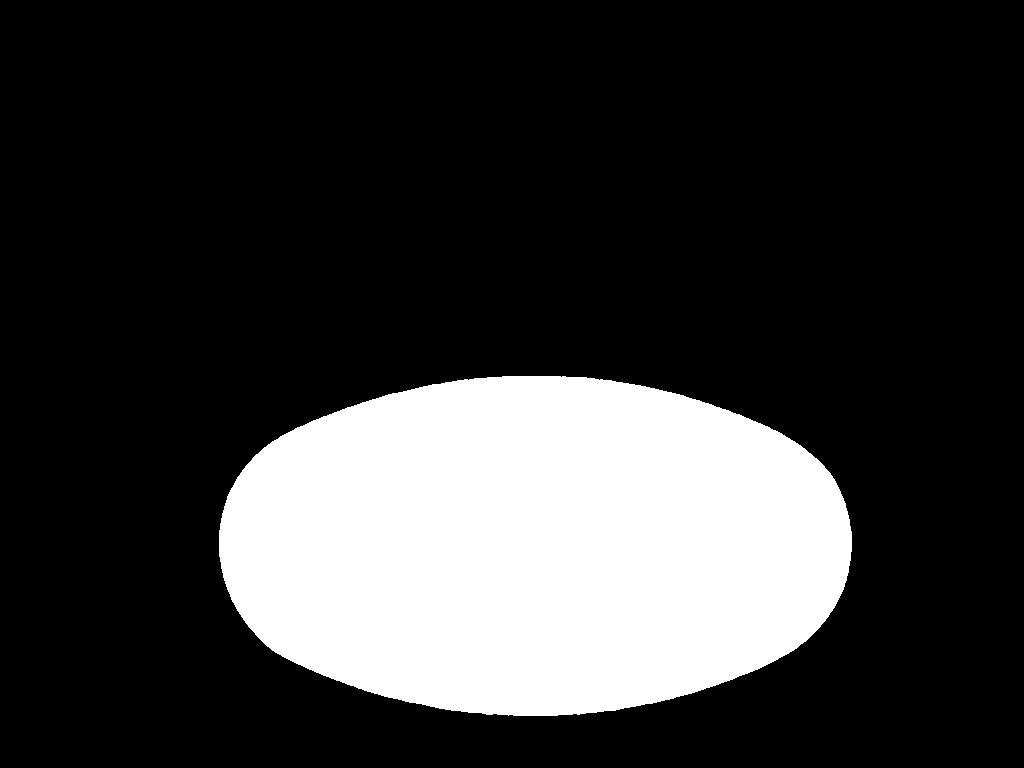
\includegraphics[width=0.3\textwidth]{figuras/processamento/mascara2.jpg}\label{fig:proMask2}}
        
        \subfloat[][Comprimido 1]{
        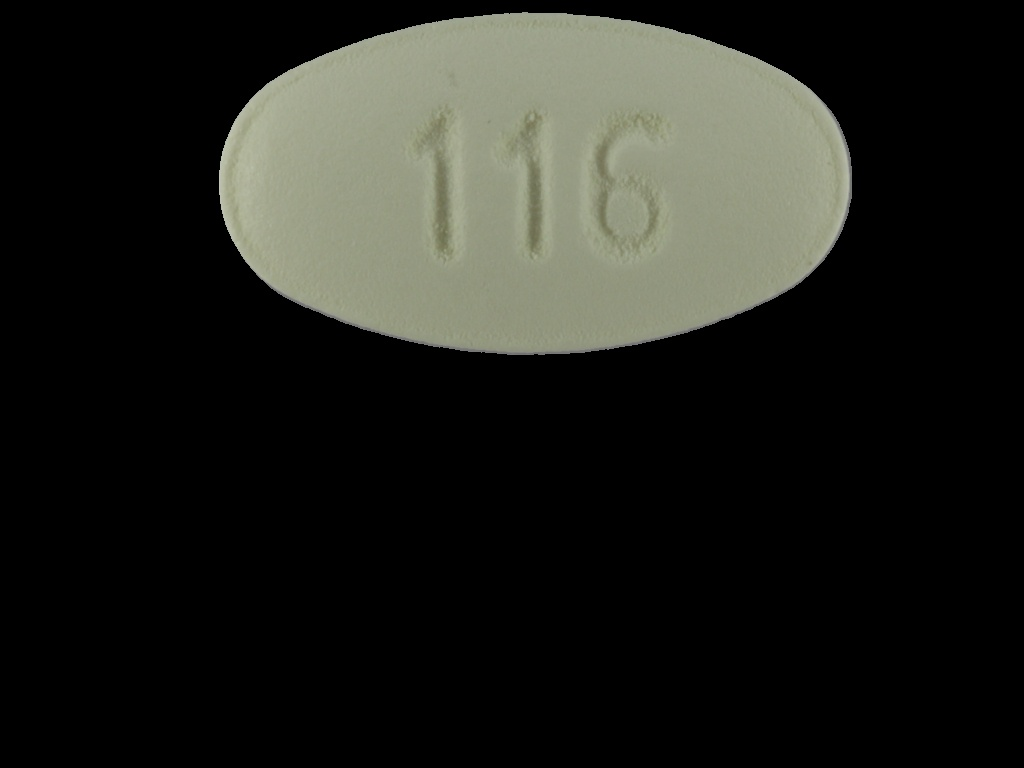
\includegraphics[width=0.3\textwidth]{figuras/processamento/pilula1.jpg}\label{fig:proPill1}}
        \subfloat[][Comprimido 2]{
        
\includegraphics[width=0.3\textwidth]{figuras/processamento/pilula2.jpg}\label{fig:proPill2}}
        
        \caption{Processo de separação}
        \label{fig:proCond}
\end{figure}

\subsection{Extração de características}

Com os comprimidos separados é possível extrair informações que serão utilizadas para classificá-los.

\begin{itemize}
    \item \textbf{Cor}
    
    Para extrair a cor do comprimido será utilizada uma média de cor de toda a região, eliminando possíveis efeitos de sombra presentes. Sendo assim, serão estabelecidos rótulos que corresponderão a uma faixa específica do espectro RGB das imagens.
    
    \newpage
    \item \textbf{Formato}
    
    Para extrair o formato do comprimido será utilizada a técnica de \textit{template matching}. Ela consiste em comparar a imagem com modelos pré-definidos, realizando a correlação da imagem com o \textit{template}, Se essa correlação for próxima de 1 significa que há uma alta probabilidade do formato estar correto. Consequentemente, é possível testar todos os formatos possíveis e identificar qual a maior correlação entre eles.
    
    \item \textbf{Texto estampado}
    
    Para extrair o texto do comprimido é necessário o tratamento da imagem para que os contornos sejam destacados com isso obtemos a figura \ref{fig:propilLim}, porém o objeto de texto ainda possui áreas não conectadas. Para contornar esse problema é utilizado uma abertura na imagem com um objeto estruturante circular pequeno com até 5 pixeis de diâmetro. Assim obtemos como resultado uma melhor definição das letras, mostrado na figura \ref{fig:propilAb}.
    
    Por fim, subtrai-se a máscara do comprimido do resultado anteriormente obtido e, consequentemente, no isolamento do texto a ser processado. O resultado da subtração da máscara pode ser visualizado na figura \ref{fig:propiltext}.
    
    Para interpretar o texto será utilizado o \textbf{Tesseract}, um sistema de reconhecimento óptico de caracteres (OCR) que utiliza uma rede neural treinada para identificar linhas de texto. Para utilização desse sistema é necessário identificar a região de interesse e isolá-la para melhores resultados. Assim obtemos o resultado na figura \ref{fig:propiltextex}, onde é possível observar a região de interesse que possui texto e o valor reconhecido.
    
    \begin{figure}[H]
        \centering
        \subfloat[][Destaque dos contornos]{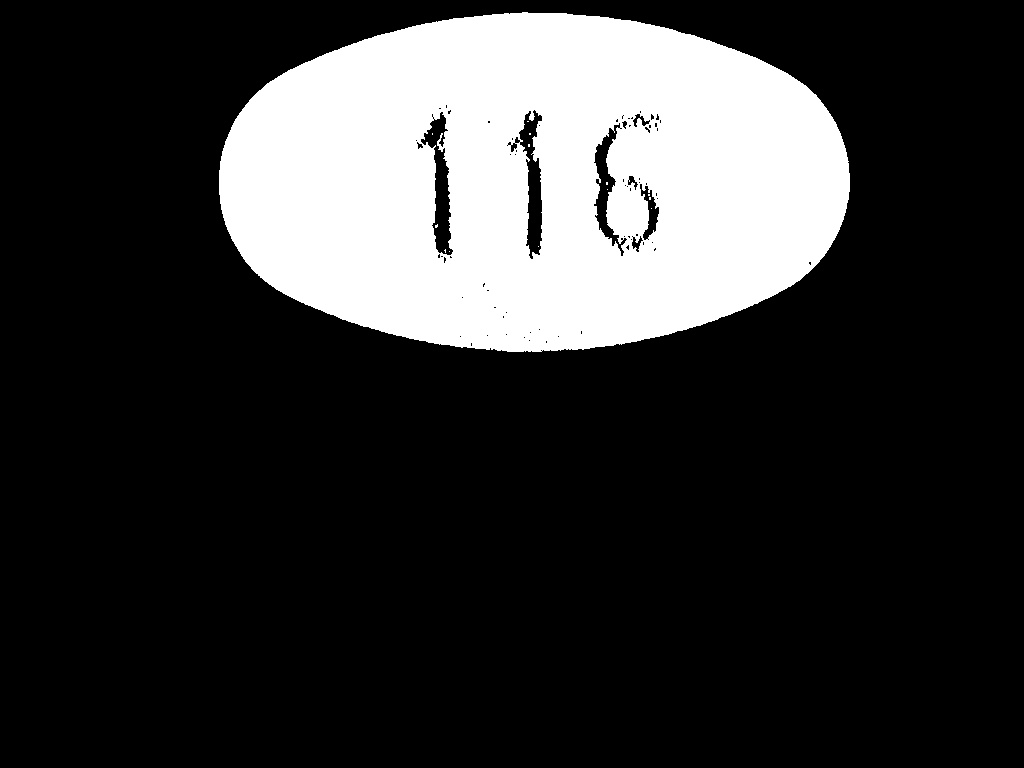
\includegraphics[width=0.3\textwidth]{figuras/processamento/pilulalimiar.jpg}\label{fig:propilLim}}
        \hspace{0.05cm}
        \subfloat[][Conexão das letras]{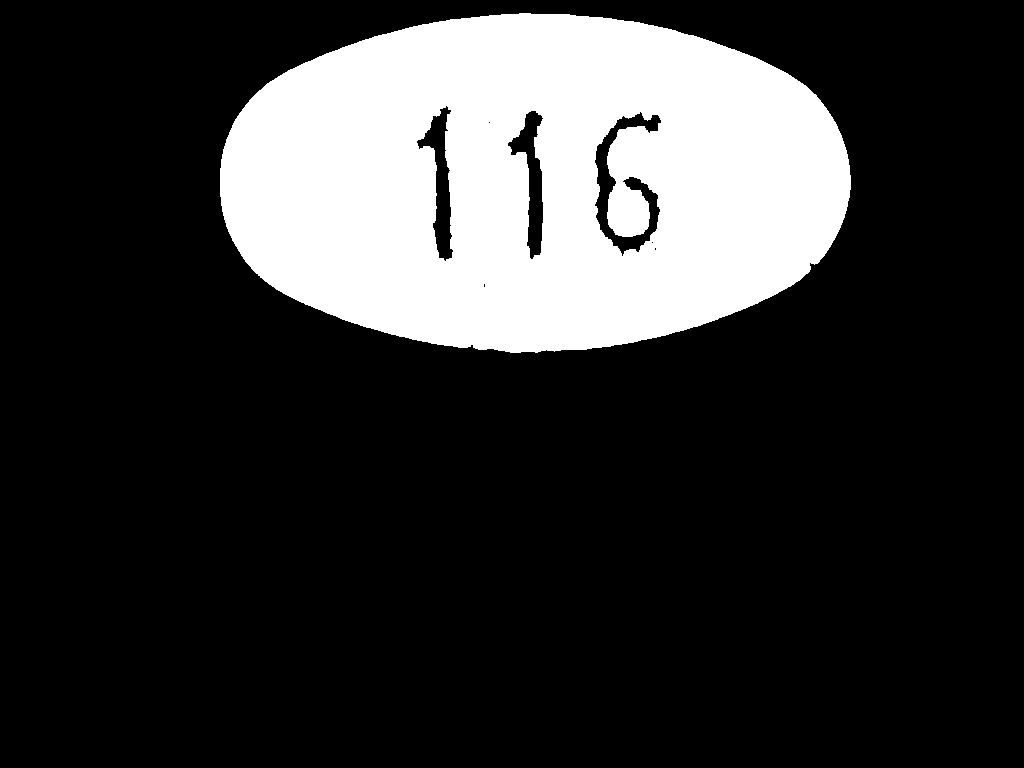
\includegraphics[width=0.3\textwidth]{figuras/processamento/pilulaabertura.jpg}\label{fig:propilAb}}
        \hspace{0.05cm}
        \subfloat[][Texto isolado]{
\includegraphics[width=0.3\textwidth]{figuras/processamento/texto.jpg}\label{fig:propiltext}}
        
        \subfloat[][Texto identificado]{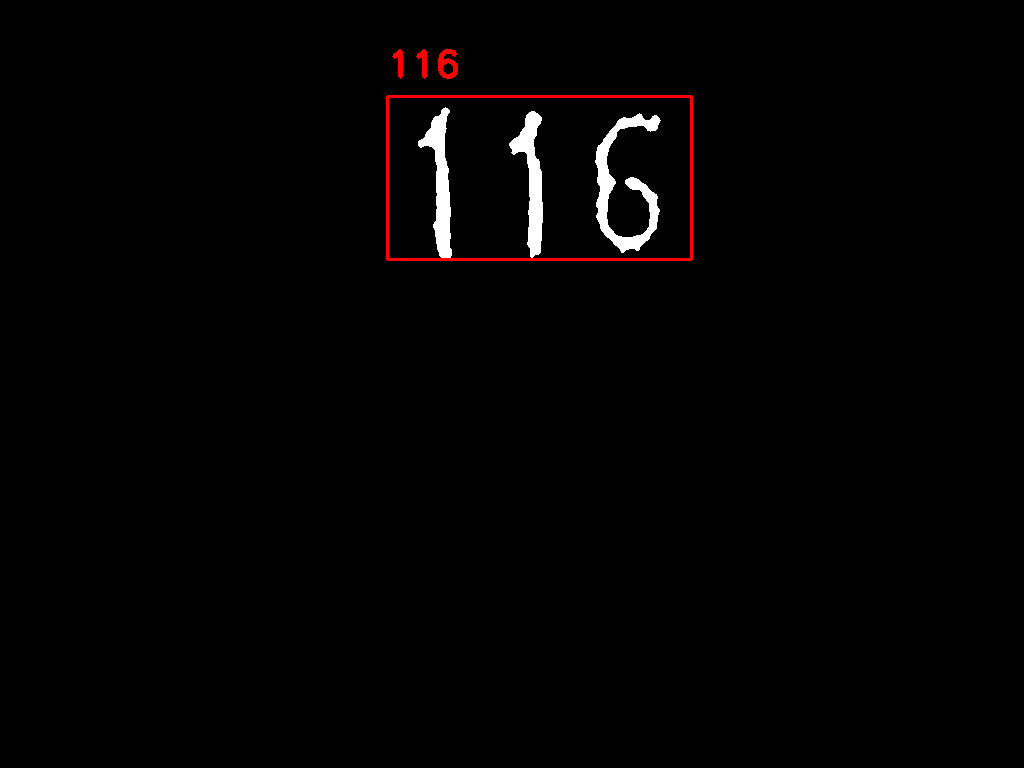
\includegraphics[width=0.4\textwidth]{figuras/processamento/textoExtraido.png}\label{fig:propiltextex}}
        
        
        \caption{Extração de texto}
        \label{fig:proText}
    \end{figure}
\end{itemize}

\subsection{Máquina de Vetores de Suporte (SVM)}

Para conseguir identificar diversos comprimidos nas imagens é necessário o uso de um classificador. Existe diversos tipos de classificos e o escolhido foi a máquina de vetores de suporte (SVM). 

Seu funcionamento se baseia na ideia de gerar uma superfície que separa as classificações por meio das características empregadas. Dessa forma são criados vetores de suporte que separam a área entre classificações, gerando assim os vetores de suporte que deve haver o treinamento da SVM.

Para o treinamento será utilizado um banco de imagens de comprimidos feito pela \textit{National Library of Medicine} que possui 4000 imagens em ambiente controlado e 133000 em imagens amadoras, disponível no  \href{https://www.nlm.nih.gov/databases/download/data_distrib_main.html}{link}. 

O tipo de classificação utilizada será a \textit{yes or no}. Na qual serão criadas SVMs para cada comprimido a ser identificado e ensinando ela para identificar características daquele comprimido.

